\documentclass[language=german,style=solution]{smo}

\usepackage{tikz}

\title{SMO - Vorrunde - Lösungen}

\begin{document}

\begin{enumerate}

\item[\textbf{1.}] 
An der SMO-Strasse stehen $n$ Häuser mit den Hausnummern 1 bis $n$, wobei $n$ eine natürliche Zahl ist. Die Häuser mit den ungeraden Nummern stehen dabei auf der linken Strassenseite, die Häuser mit den geraden Nummern auf der rechten. Der Postbote Quirin möchte jedem Haus eine Zeitung vorbeibringen. Wie viele Möglichkeiten hat er, dies zu tun, wenn er nach jeder abgegebenen Zeitung die Strassenseite wechseln möchte?

\textbf{Lösung}

Wir unterscheiden zwischen $n$ gerade und $n$ ungerade:

\begin{minipage}{0.08\textwidth}
\mbox{}
\end{minipage}
\begin{minipage}{0.86\textwidth}
\begin{enumerate}
\item[$n$ gerade:] In diesem Fall gibt es auf beiden Strassenseiten gleich viele Häuser. Quirin kann also zuerst eine Strassenseite wählen. Auf der gewählten Strassenseite hat er nun $\frac{n}{2}$ Häuser zur Auswahl. Nachdem er dort die Zeitung abgegeben hat, kann er auf der anderen Strassenseite wieder zwischen $\frac{n}{2}$ Häusern auswählen. Danach wechselt er die Strassenseite, und steht somit wieder auf der Seite, auf der er begonnen hat. Hier hat er aber nur noch $\frac{n}{2}-1$ Möglichkeiten, da er ja bereits eine Zeitung verteilt hat. Nun wechselt er wieder die Strassenseite, usw. Somit hat Quirin insgesamt
$2 \cdot \frac{n}{2} \cdot \frac{n}{2} \cdot (\frac{n}{2}-1)\cdot ... \cdot 1 = 2\cdot(\frac{n}{2}!)^2$ Möglichkeiten, wenn $n$ gerade ist.
\item[$n$ ungerade:] In diesem Fall stehen auf der linken Strassenseite $\frac{n+1}{2}$ Häuser und auf der rechten nur $\frac{n-1}{2}$. Somit muss Quirin auf der linken Seite anfangen, die Zeitungen zu verteilen, ansonsten kann er nicht nach jeder abgegebenen Zeitung die Seite wechseln. Ähnlich wie oben erhält man also
$\frac{n+1}{2} \cdot \frac{n-1}{2}\cdot \frac{n-1}{2}\cdot \ldots \cdot 1 = \frac{n+1}{2}\cdot (\frac{n-1}{2}!)^2$ Möglichkeiten, falls $n$ ungerade ist.
\end{enumerate}
\end{minipage}

\textbf{Marking Scheme}

+1 Für die Beobachtung, dass Quirin im ungeraden Fall links anfangen muss.\\
+2 Wenn man \emph{zusätzlich} sieht, dass Quirin geraden Fall die Wahl hat.

+2 Für das richtige Zählen pro Fall (ungerade / gerade).\\
-1 Pro kleinem Fehler (z.B. den Faktor 2 im geraden Fall vergessen).\\
Wenn man nicht zwischen gerade und ungerade unterscheidet, kann man maximal 4 Punkte erhalten. 

\newpage

\item[\textbf{2.}] 
Für welche natürlichen Zahlen $n$ ist es möglich, ein $n\times n$ Feld lückenlos und überlappungsfrei mit T-Tetrominos und einer ungeraden Anzahl an Square-Tetrominos zu bedecken?
\vspace{-0cm}
\begin{center}
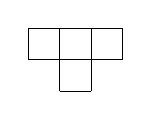
\begin{tikzpicture}[scale=0.4]
\draw (0,1) grid (3,2);
\draw (1,0) grid (2,1);
\end{tikzpicture}
\quad
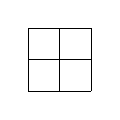
\begin{tikzpicture}[scale=0.4]
\draw (0,0) grid (2,2);
\end{tikzpicture}
\end{center}
\textit{Bemerkung: Es ist erlaubt, keine T-Tetrominos zu verwenden.}


\textbf{Lösung:}

Puisque les deux pièces à disposition comportent chacune 4 cases, on obtient que le nombre total de cases est divisible par 4. Comme ce nombre vaut $n^2$, $4 | n^2$, donc $2 | n $. Posons $n = 2k$.\\
En utilisant la coloration standard à deux couleurs (également appelée coloration de l'échiquier), on remarque que chaque Square-Tetromino recouvre 2 cases noires et 2 cases blanches, et les T-Tetrominos recouvrent soit 3 cases noires et une case blanche, soit 3 cases blanches et une case noire. Puisque $n$ est pair, il y a autant de cases blanches que de cases noires, et donc il doit y avoir autant de T-Tetrominos des deux sortes.\\
Il y a donc forcément un nombre pair de T-Tetrominos, et la donnée nous indique qu'on doit utiliser un nombre impair de Square-Tetrominos, donc en tout nous avons un nombre impair de pièces. Soit $m$ ce nombre de pièces. Comme chaque pièce contient 4 cases, il doit donc y avoir en tout $4m$ cases. Or, le nombre de cases total vaut $n*n$, soit $4k^2$. Autrement dit, $k^2 = m$, donc $k^2$ est impair. Puisque $k^2$ est impair, $k$ lui-même doit être impair.\\
Nous obtenons ainsi que les seules solutions possibles sont de la forme $n = 2k$ avec $k$ un nombre impair. Nous allons maintenant voir que pour chaque $k$ impair, il est possible de remplir l'échiquier $2k\times 2k$ en respectant la consigne.\\
Pour cela, il suffit de paver l'échiquier avec des Square-Tetrominos. En effet, puisque $n$ est pair, il est possible de paver l'échiquier avec des Square-Tetrominos, et vu que chaque pièce contient 4 cases, on utilise $\frac{2k*2k}{4} = k^2$ Square-Tetrominos; $k^2$ est impair puisque $k$ est impair.

\textbf{Marking Scheme:}

\begin{itemize}
\item Déduire par une coloration appropriée que le nombre de T-Tetromino est pair: +3 points
\item En conclure que $k$ est impair: +3 points
\item La construction pour $k$ impair: +1 point
\end{itemize}

Une construction non justifiée ne rapporte aucun point. Pour obtenir des points sur la construction, il faut avoir prouvé que k est impair.

\newpage

\item[\textbf{3.}]
Finde alle Tripel $(a,b,c)$ natürlicher Zahlen, sodass
\[
\frac{a+b}{c},\frac{b+c}{a},\frac{c+a}{b}
\]
%\[
%c \,|\, a+b \qquad a \,|\, b+c \qquad b \,|\, a+c
%\]
ebenfalls natürliche Zahlen sind.

\textbf{Lösung 1:}

Wir unterscheiden drei Fälle, und zwar, dass die drei Zahlen gleich sind, dass zwei der drei Zahlen gleich sind und dass die drei Zahlen verschieden sind.

\begin{minipage}{0.02\textwidth}
\mbox{}
\end{minipage}
\begin{minipage}{0.93\textwidth}
\begin{enumerate}
\item[Fall 1:] $a=b=c$\\
Dies ergibt die Lösung $(a,a,a)$.
\item[Fall 2:] Wir haben zwei gleiche und eine andere Zahl.\\
Nehme an, dass $a=b\neq c$. Einsetzen führt zu $a\mid a+c$. Wir erhalten $a \mid c$. $c$ ist also ein Vielfaches von $a$. Ebenfalls einsetzen führt zu $c \mid a+a$, also $c \mid 2a$. Somit muss $c=a$ oder $c=2a$ gelten. Die erste Möglichkeit haben wir in Fall 1 betrachtet, die zweite Möglichkeit liefert die Lösung $(a,a,2a)$.
\item[Fall 3:] Wir haben drei verschiedene Zahlen.\\
Nehme an, dass $a < b < c$ gilt. Insbesondere gilt dann $a+b<2c$. Ausserdem wissen wir, dass $c\mid a+b$. Dies ist nur möglich, wenn $c=a+b$ gilt. Somit können wir die Bedingung $b\mid c+a$ umschreiben zu $b\mid a+b+a$, woraus $b\mid 2a$ folgt. Da nach Annahme $a<b$ gilt, ist dies nur möglich, wenn wir $b=2a$ haben. Daraus folgt $c=3a$ und wir erhalten die Lösung $(a,2a,3a)$.\\
Insgesamt erhalten wir also die Lösungen $(a,a,a)$, $(a,a,2a)$, $(a,2a,3a)$ und die symmetrischen Vertauschungen davon, wobei $a$ jede natürliche Zahl sein darf. Einsetzen liefert, dass jedes dieser Tripel auch tatsächlich eine Lösung ist.
\end{enumerate}
\end{minipage}

\textbf{Lösung 2:}

Nehme an, dass $c\geq b \geq a$. Wir wissen nun, dass $c\mid a+b$ und $a+b\leq 2c$. Daraus folgt, dass entweder $c=a+b$ oder $2c=a+b$. Wir betrachten diese beiden Fälle einzeln.\\
Fall 1: $2c=a+b$\\
Da $a\leq b\leq c$ gilt, ist dies nur möglich für $a=b=c$. Wir bekommen also die Lösung $(a,a,a)$.\\
Fall 2: $c=a+b$\\
Es gilt $b\mid a+c$, also $b\mid a+a+b$ und folglich $b\mid 2a$. Da $b\geq a$, muss $b=a$ oder $b=2a$ gelten. Dies führt zu den Lösungen $(a,a,2a)$ und $(a,2a,3a)$.\\
Insgesamt erhalten wir also die Lösungen $(a,a,a)$, $(a,a,2a)$, $(a,2a,3a)$ und die symmetrischen Vertauschungen davon, wobei $a$ jede natürliche Zahl sein darf. Einsetzen liefert, dass jedes dieser Tripel auch tatsächlich eine Lösung ist.

\textbf{Marking Scheme:}

+1 P für $c$ als grösste Zahl wählen und sinnvolle Fallunterscheidung (``Strategiepunkt'')\\
+1 für $c\mid a+b$, $c$ grösste Zahl, also $a+b=c$ oder $a+b=2c$. (Zweite Gleichung nur erwartet, falls sie im momentanen Fall möglich ist.)

Falls eine sinnvolle Fallunterscheidung gemacht wird:\\
+1 für Fall 1\\
+1 für Fall 2 in Lösung 1\\
+3 für Fall 2 in Lösung 2\\
+3 für Fall 3 in Lösung 1 (ein Punkt davon ist für $a+b=c$)\\
-1, falls komplette Lösung, aber symmetrische Vertauschungen vergessen.\\

\newpage

\item[\textbf{4.}] 
Sei $ABC$ ein spitzwinkliges Dreieck und $W$ der Schnittpunkt der Winkelhalbierenden von $\angle ACB$ und der Seite $AB$. Weiter seien $I_A$ und $I_B$ die Inkreismittelpunkte der Dreiecke $AWC$ respektive $WBC$. Die Geraden $I_AW$ und $I_BB$ schneiden sich im Punkt $D$. Sei $M$ der Mittelpunkt der Strecke $DI_B$.
Zeige, dass $MWBC$ ein Sehnenviereck ist.

\textit{Bemerkung: Die drei Winkelhalbierenden eines Dreiecks schneiden sich in einem Punkt, dem Inkreismittelpunkt.}

\textbf{Lösung 1:}

Die Geraden $WI_A$ und $WI_B$ halbieren die Winkel $\angle CWA$ und $\angle BWC$, folglich gilt:
\[
\angle I_BWD=\angle I_BWC+\angle CWI_A=\frac{1}{2}(\angle BWC+\angle CWA)=90^\circ.
\]
Somit liegt $W$ auf dem Thaleskreis über $DI_B$, dessen Mittelpunkt $M$ ist.\\
Mit den Winkelhalbierenden $WD$ und $BD$ und mit dem Aussenwinkelsatz in den Dreiecken $WBC$ und $WBD$ folgt:
\begin{align*}
\angle CBW+\angle WCB &=\angle CWA\\
&=2\angle DWA\\
&=2\left(\angle DBW+\angle WDB\right)\\
&=\angle CBW+2\angle WDB.
\end{align*}
Hieraus folgt sofort $2\angle WDB=\angle WCB$. Mit dem Mittelpunktswinkelsatz erhalten wir nun:
\[
\angle WMB=\angle WMI_B=2\angle WDI_B=2\angle WDB=\angle WCB.
\]
Damit ist gezeigt, dass $MWBC$ ein Sehnenviereck ist.

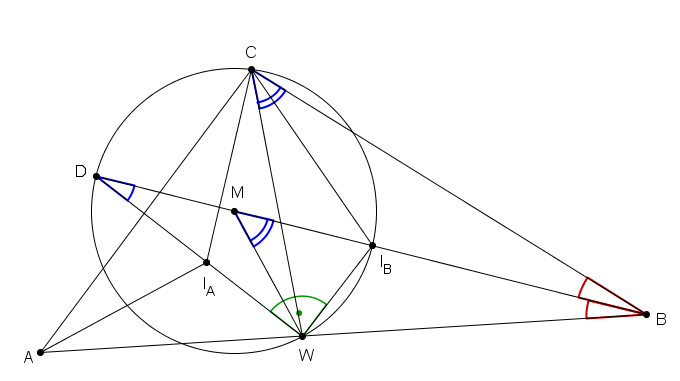
\includegraphics{muleo_2015.PNG}
\newpage
\textbf{Lösung 2:}

Wie oben erhalten wir $\angle I_BWD=90^\circ$. $D$ liegt auf den Winkelhalbierenden von $\angle CWA$ und $\angle CBA$, folglich hat $D$ denselben Abstand zu den Geraden $WC$ und $WA$ und auch denselben Abstand zu den Geraden $BC$ und $BA$. Da aber $WA$ die gleiche Gerade ist wie $BA$, folgt hieraus, dass $D$ auch zu den Geraden $WC$ und $BC$ denselben Abstand hat. Das bedeutet, dass $D$ auf der Winkelhalbierenden des Aussenwinkels von $\angle WCB$ liegt.
Analog wie oben können wir nun folgern, dass $\angle DCI_B=90^\circ$ gilt. $W$ und $C$ liegen somit beide auf dem Thaleskreis über $DI_B$, dessen Mittelpunkt $M$ ist.\\
Mit dem Mittelpunktswinkelsatz und der Winkelhalbierenden $CI_B$ folgt nun:
\[
\angle WMB=\angle WMI_B=2\angle WCI_B=\angle WCB.
\]
Damit ist gezeigt, dass $MWBC$ ein Sehnenviereck ist.\\

\textbf{Marking Scheme:}

1 Punkt, falls eine der folgenden Aussagen gezeigt wurde:
\begin{enumerate}[1)]
\item $W$ liegt auf dem Thaleskreis über $DI_B$.
\item $C$ liegt auf dem Thaleskreis über $DI_B$.
\item $W$ und $C$ liegen beide auf dem Thaleskreis über $DI_B$.
\item $DWI_BC$ ist ein Sehnenviereck.
\end{enumerate}
Falls obige Aussage gezeigt wurde, gab es 3 weitere Punkte für die Beobachtung, dass der Mittelpunkt dieses (Thales-)Kreises $M$ ist.

\newpage

\item[\textbf{5.}] 
Den unten abgebildeten Spielstein nennen wir eine Treppe. Für welche Paare $(m,n)$ natürlicher Zahlen mit $m,n\geq 6$ ist es möglich, ein $m\times n$ Feld lückenlos und überlappungsfrei mit Treppen zu bedecken?
\vspace{-0cm}
\begin{center}

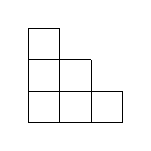
\begin{tikzpicture}[scale=0.4]
\draw (-1,0) grid (2,1);
\draw (-1,1) grid (1,2);
\draw (-1,2) grid (0,3);
\end{tikzpicture}
\quad
\end{center}

\textbf{Lösung:}

Comme l'escalier a une taille de $6$, on conclue que $6|mn$ et donc, sans perte de généralité, $2|n$. Faisons une coloration par ligne en deux couleurs (noir et blanc) perpendiculaire au côté de longueur paire. Il y a donc autant de cases noires que de cases blanches. Or chaque escalier couvre quatre cases d'une couleur et deux de l'autre. On en déduit qu'il faut utiliser un nombre pair d'escaliers et donc $12|mn$.\\
\\Distinguons trois cas :
\begin{enumerate}
\item $4|n$ et $3|m$\\
Dans ce cas, on recouvre le rectangle entièrement avec le petit rectangle de taille $3\times 4$ constitué de deux escaliers.
\item $12|n$\\
Dans ce cas, on peut écrire $m=4k_1 +3k_2$ et $k_1,k_2\geq 0$ et on peut à nouveau recouvrir notre rectangle avec des petits rectangles $3\times 4$ constitués de deux escaliers. En effet, on peut séparer notre rectangle $m\times n$ en deux rectangles $4k_1\times n$ et $3k_2\times n$, tous deux recouvrables facilement avec des rectangles $3\times 4$, car $12|n$.
\item ($6|n$ et $2|m$) ou ($2|n$ et $6|m$)\\
Dans ce cas, les deux longueurs sont paires et on applique une coloration en quatre couleurs :
\begin{center}
1-2-1-2-1-2-...\\
3-4-3-4-3-4-...\\
1-2-1-2-1-2-...\\
...
\end{center}
Ainsi, dans chaque carré $2\times 2$ on retrouve les quatre couleurs. Un escalier recouvre trois cases d'une couleur et trois autres cases des trois autres couleurs. Ainsi le nombre d'escaliers qu'il faut utiliser est un multiple de quatre et donc $24|mn$. On en déduit que au moins un des côtés est divisible par quatre et on se ramène au deux cas précédents.
\end{enumerate}
Au final, on a les solutions : $(12a,b)$ et $(3c,4d)$ où $a\geq 1, b\geq 6, c\geq 2$ et $d\geq 3$ (et leurs permutations). 

\textbf{Marking Scheme:}

Preuver 12|mn: 1pt
\begin{enumerate}[a)]
\item le cas 4|n et 3|m : 0 pt
\item le cas 12|n : 1 pt
\item le cas 2|n et 2|m : 5 pts
\end{enumerate}

-1 pt : oublier les permutations des solutions\\
-1 pt: fait les cas b) et c) et avoir oublié a)

\end{enumerate}

\end{document}
